%! Author = angela
%! Date = 24/01/24
% !TeX root = ../thesis-main.tex

\chapter{Validation}
\label{ch:validation}
This chapter describes the validation process of the new \ac{dsl} implementation and incarnation.
Validating the hypotheses is a fundamental step for the correct evaluation of the work done.
It is divided into testing and performance comparison, which are the two main aspects of this validation process.
By comparing the performance of the new implementation with the original one, it is possible to understand if the
introduction of the new features has led to an improvement in the performance of the system.

\section{Tests}
\label{sec:tests}
The testing phase is instrumental in affirming the integrity and functionality of the \ac{dsl} codebase developed for this thesis.
Tests serve as a critical mechanism for verifying the behaviour of the DSL across various scenarios, detecting potential bugs,
and validating adherence to specifications.

Since the \ac{dsl} is designed to be multiplatform, tests are written to ensure that the codebase is compatible with
different platforms and the results across platforms must be consistent.

To achieve this, Kotlin offers \emph{Multiplatform Extensions}, which allows the testing of the same codebase across
different platforms, such as \emph{JVM}, \emph{JS}, and \emph{Native}, just by adding needed extensions in the \texttt{build.gradle} file.
%sono i seguenti
The targets chosen for the testing are the following:
\begin{itemize}
    \item Linux x64 and ARM64;
    \item Windows x64(MinGW);
    \item MacOS x64 and ARM64;
    \item IOS x64 and (simulator) ARM64;
    \item WatchOS x64 and (simulator) ARM64;
    \item TvOS x64 and (simulator) ARM64;
\end{itemize}

Those were chosen to cover the most common platforms and to ensure that the \ac{dsl} is compatible with the most common
devices, such as smartphones, tablets, and wearables.
Test have been implemented using the \emph{Kotest} framework, which is a flexible and comprehensive testing framework for Kotlin
with multiplatform support.

\paragraph{Unit Tests}
Focused on individual units or components within a software system, unit testing serves to validate their functionality
according to requirements.
Typically conducted by developers as the initial testing phase, it involves automation and occurs each time modifications
are made to the source code to prevent disruption of existing features.
These tests are engineered to verify the smallest units of code, such as individual functions or methods, in isolation
from the broader system context.

\paragraph{Integration Tests}
Integration testing is a software testing methodology used to evaluate the functionality of combined units of code.
It serves to expose faults in the interaction between integrated units, ensuring that they function as expected.
This type of testing is particularly useful in the context of the \ac{dsl} as it allows the verification of the correct
interactions of the different parts of the system.

\subsection{Continuous Integration and Deployment}
\label{subsec:continuous-integration-and-deployment}
\ac{cicd} are software development practices that aim to automate and streamline the process of delivering high-quality software.
\ac{ci} is a development practice where developers frequently integrate their code changes into a shared repository.
Each integration triggers an automated build process, during which the code is compiled, tested, and verified against a
set of predefined criteria.

The primary goals of \ac{ci} are to detect integration errors early, ensure that the codebase remains functional,
and promote collaboration among team members.
\ac{ci} key features include:
    i) automated builds, automatically triggered by committed code changes;
    ii) automated testing, run automatically during the build process;
    iii) immediate feedback, provided to developers regarding the status of their code changes, allowing to address issues promptly;
    iv) version control integration, enabling seamless integration with code repositories.

\ac{cd} extends the principles of \ac{ci} by automating the deployment process after successful integration and testing.
It involves automatically deploying validated code changes to production or staging environments, eliminating manual
intervention and reducing the time between code changes and their availability to users.
\ac{cd} helps streamline the release process, reduce deployment errors, and enable rapid and reliable software delivery.
\ac{cd} key features include:
    i) automated deployment, Deployments to production or staging environments are automated, ensuring consistency and reliability;
    ii) continuous monitoring, integrated into CD pipelines to track application performance and detect issues in real-time;
    iii) rollback mechanisms, in case of deployment failures;
    iv) environment provisioning, pipelines often include steps for provisioning and configuring target environments as part of the deployment process.

\section{Alchemist Simulations}
\label{sec:alchemist-simulations}
Another validation process regards the effective functioning of \emph{Collektive Incarnation} for the \emph{Alchemist} simulator.
To see if the new incarnation is working as expected, examples of simulations have been implemented and run.

Using the Alchemist Simulator for validation showcases the capability of Collektive: implementing algorithms to specify
system behavior is straightforward, and execution is both swift and dependable.

\paragraph{Neighbour Counter}
The first example is a simple aggregate program in which the devices count the number of neighbours they have (\Cref{lst:neighbour-counter-example}).
The result is a map of the space in which each node has a value that represents the number of neighbours it has.

\begin{lstlisting}[language=kt, caption={Neighbour counter code example}, label={lst:neighbour-counter-example}]
fun Aggregate<Int>.neighborCounter(): Int = neighboringViaExchange(1)
    .hood(0) { acc, _ -> acc + 1 }
\end{lstlisting}

The resultant simulation appears at first empty, because the nodes are coloured with a gradient that goes from white to
blue based on the number of neighbours they have.
Once the simulation starts and the nodes communicate with each other, the space is filled with colours, and the number of
neighbours and connections is visible, as shown in \Cref{fig:neighbour-counter}.

\begin{figure}[ht!]
    \centering
    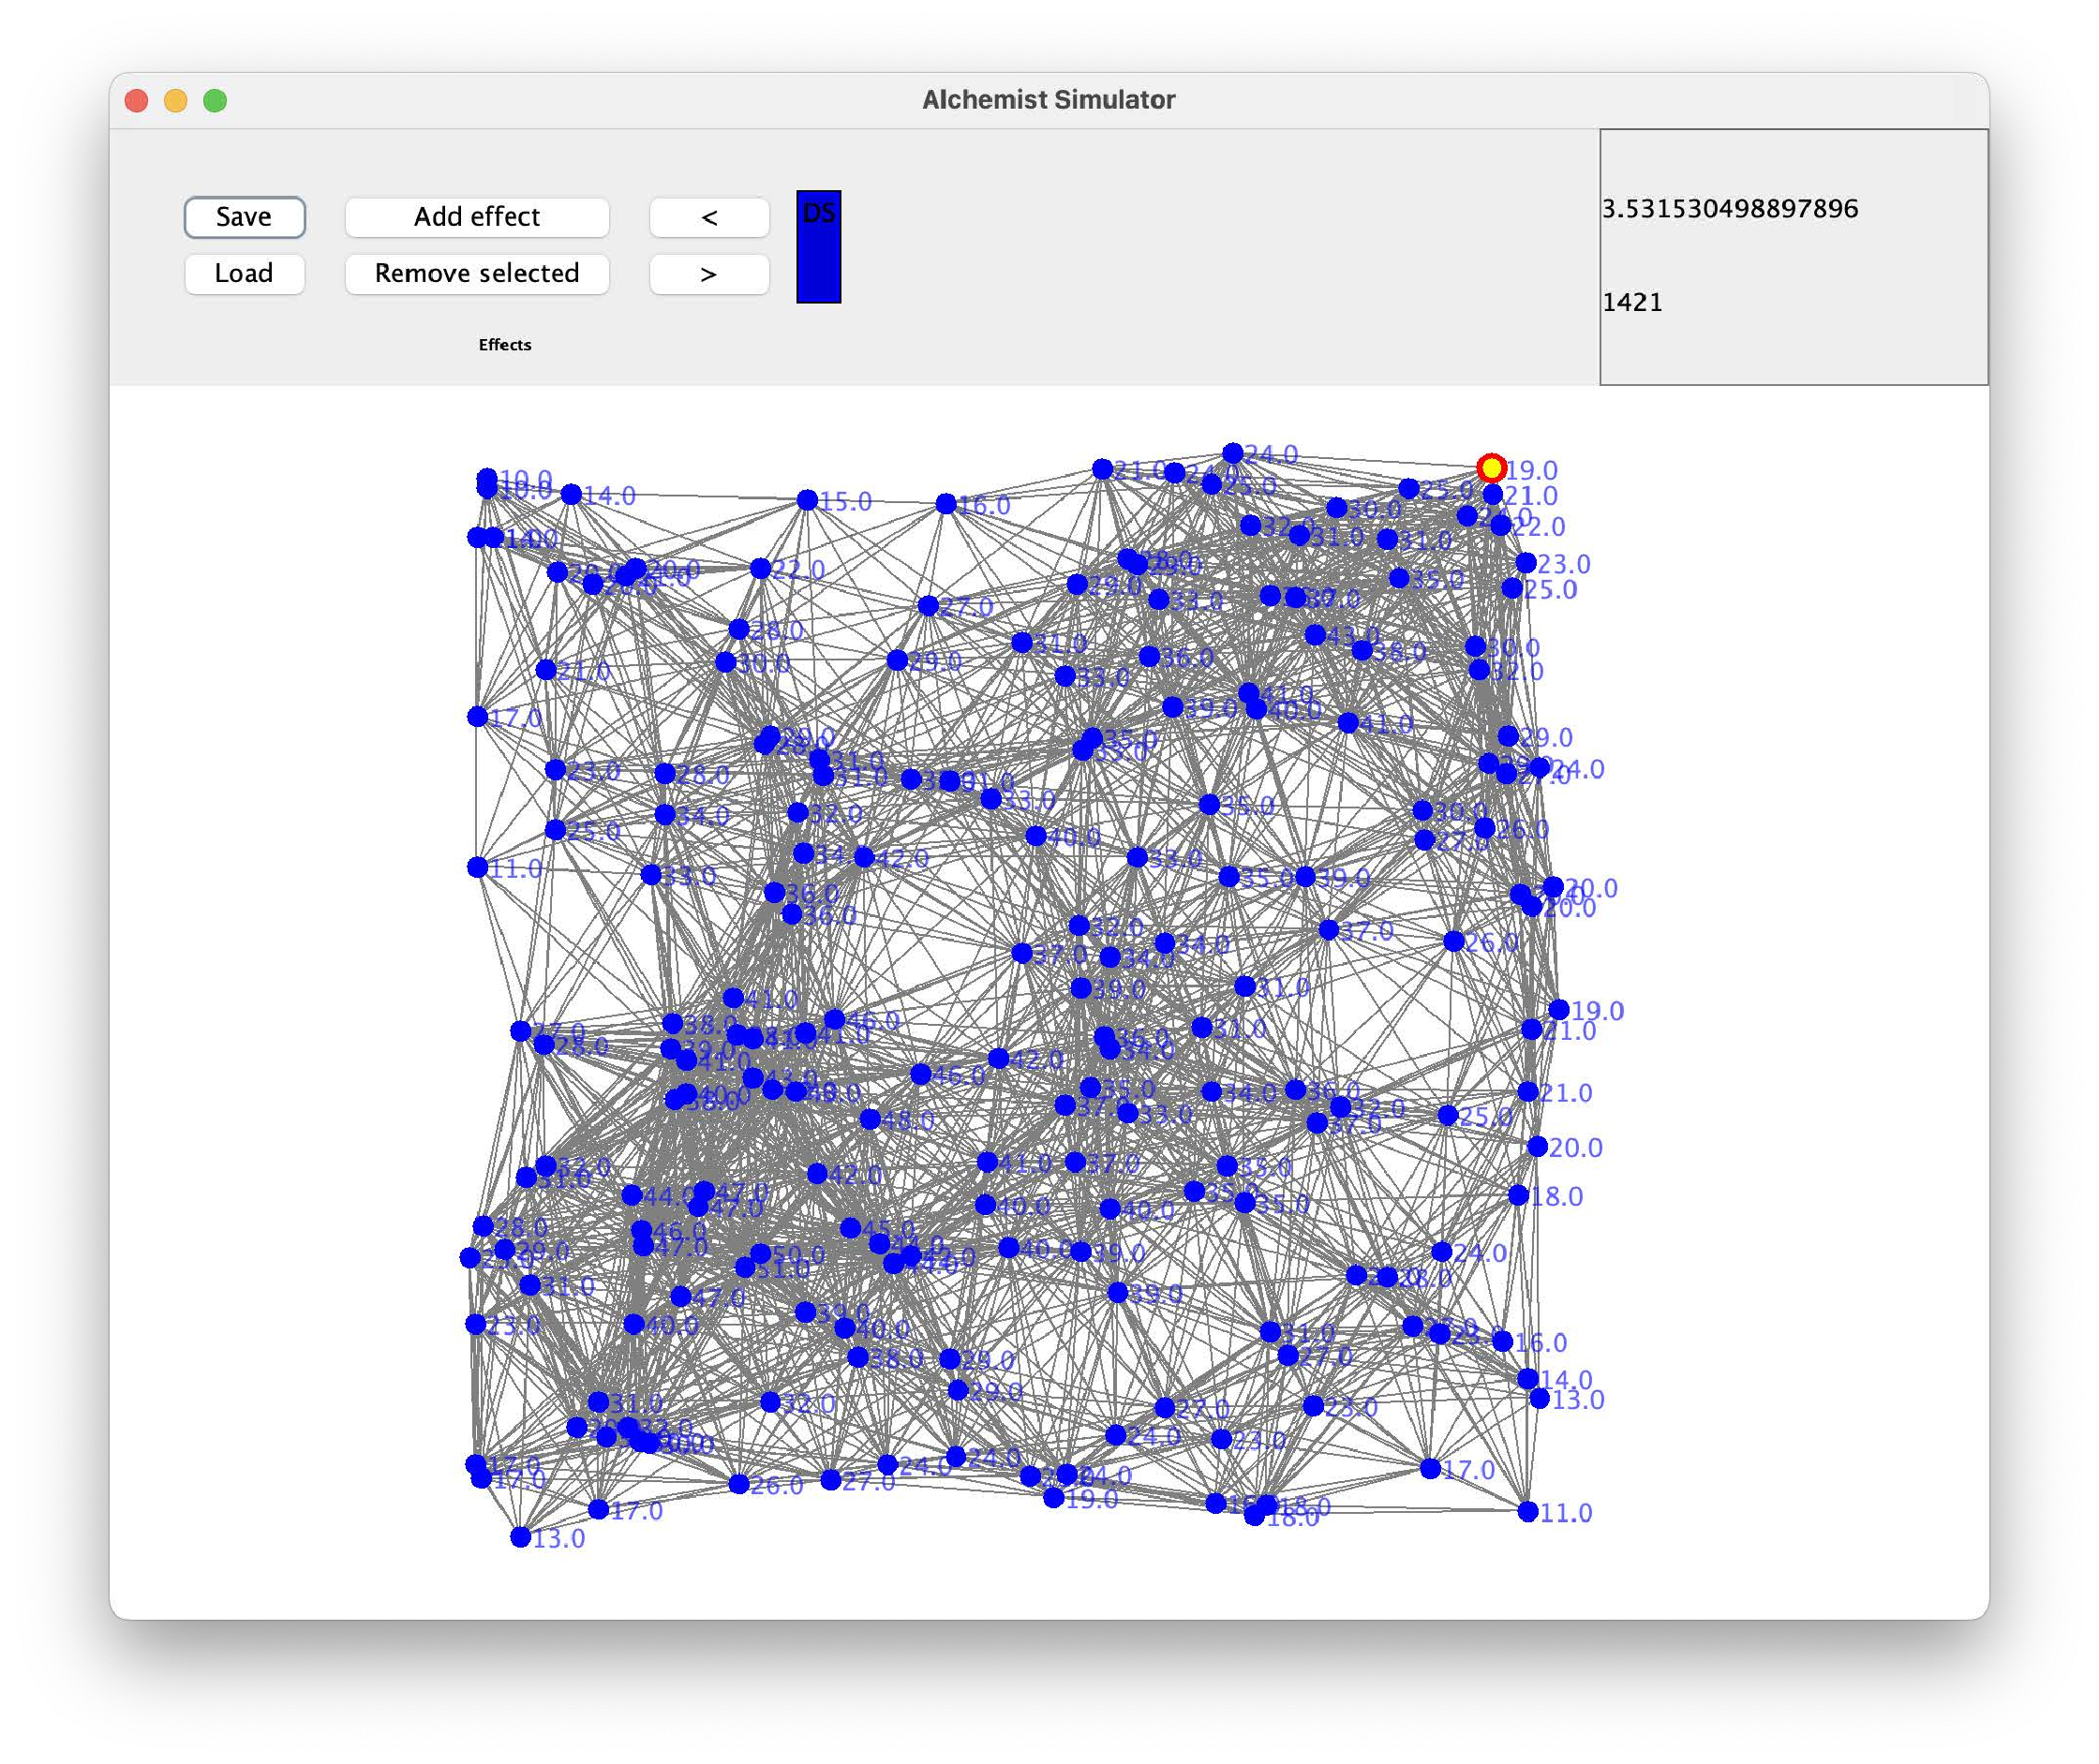
\includegraphics[width=0.8\textwidth]{figures/neighborCounter}
    \caption{Neighbour Counter Simulation.}
    \label{fig:neighbour-counter}
\end{figure}

The simulator also gives the opportunity to move the nodes around the environment, and the number of neighbours is updated
in real-time, as shown in \Cref{fig:neighbor-counter-moved}.
\begin{figure}[ht!]
    \centering
    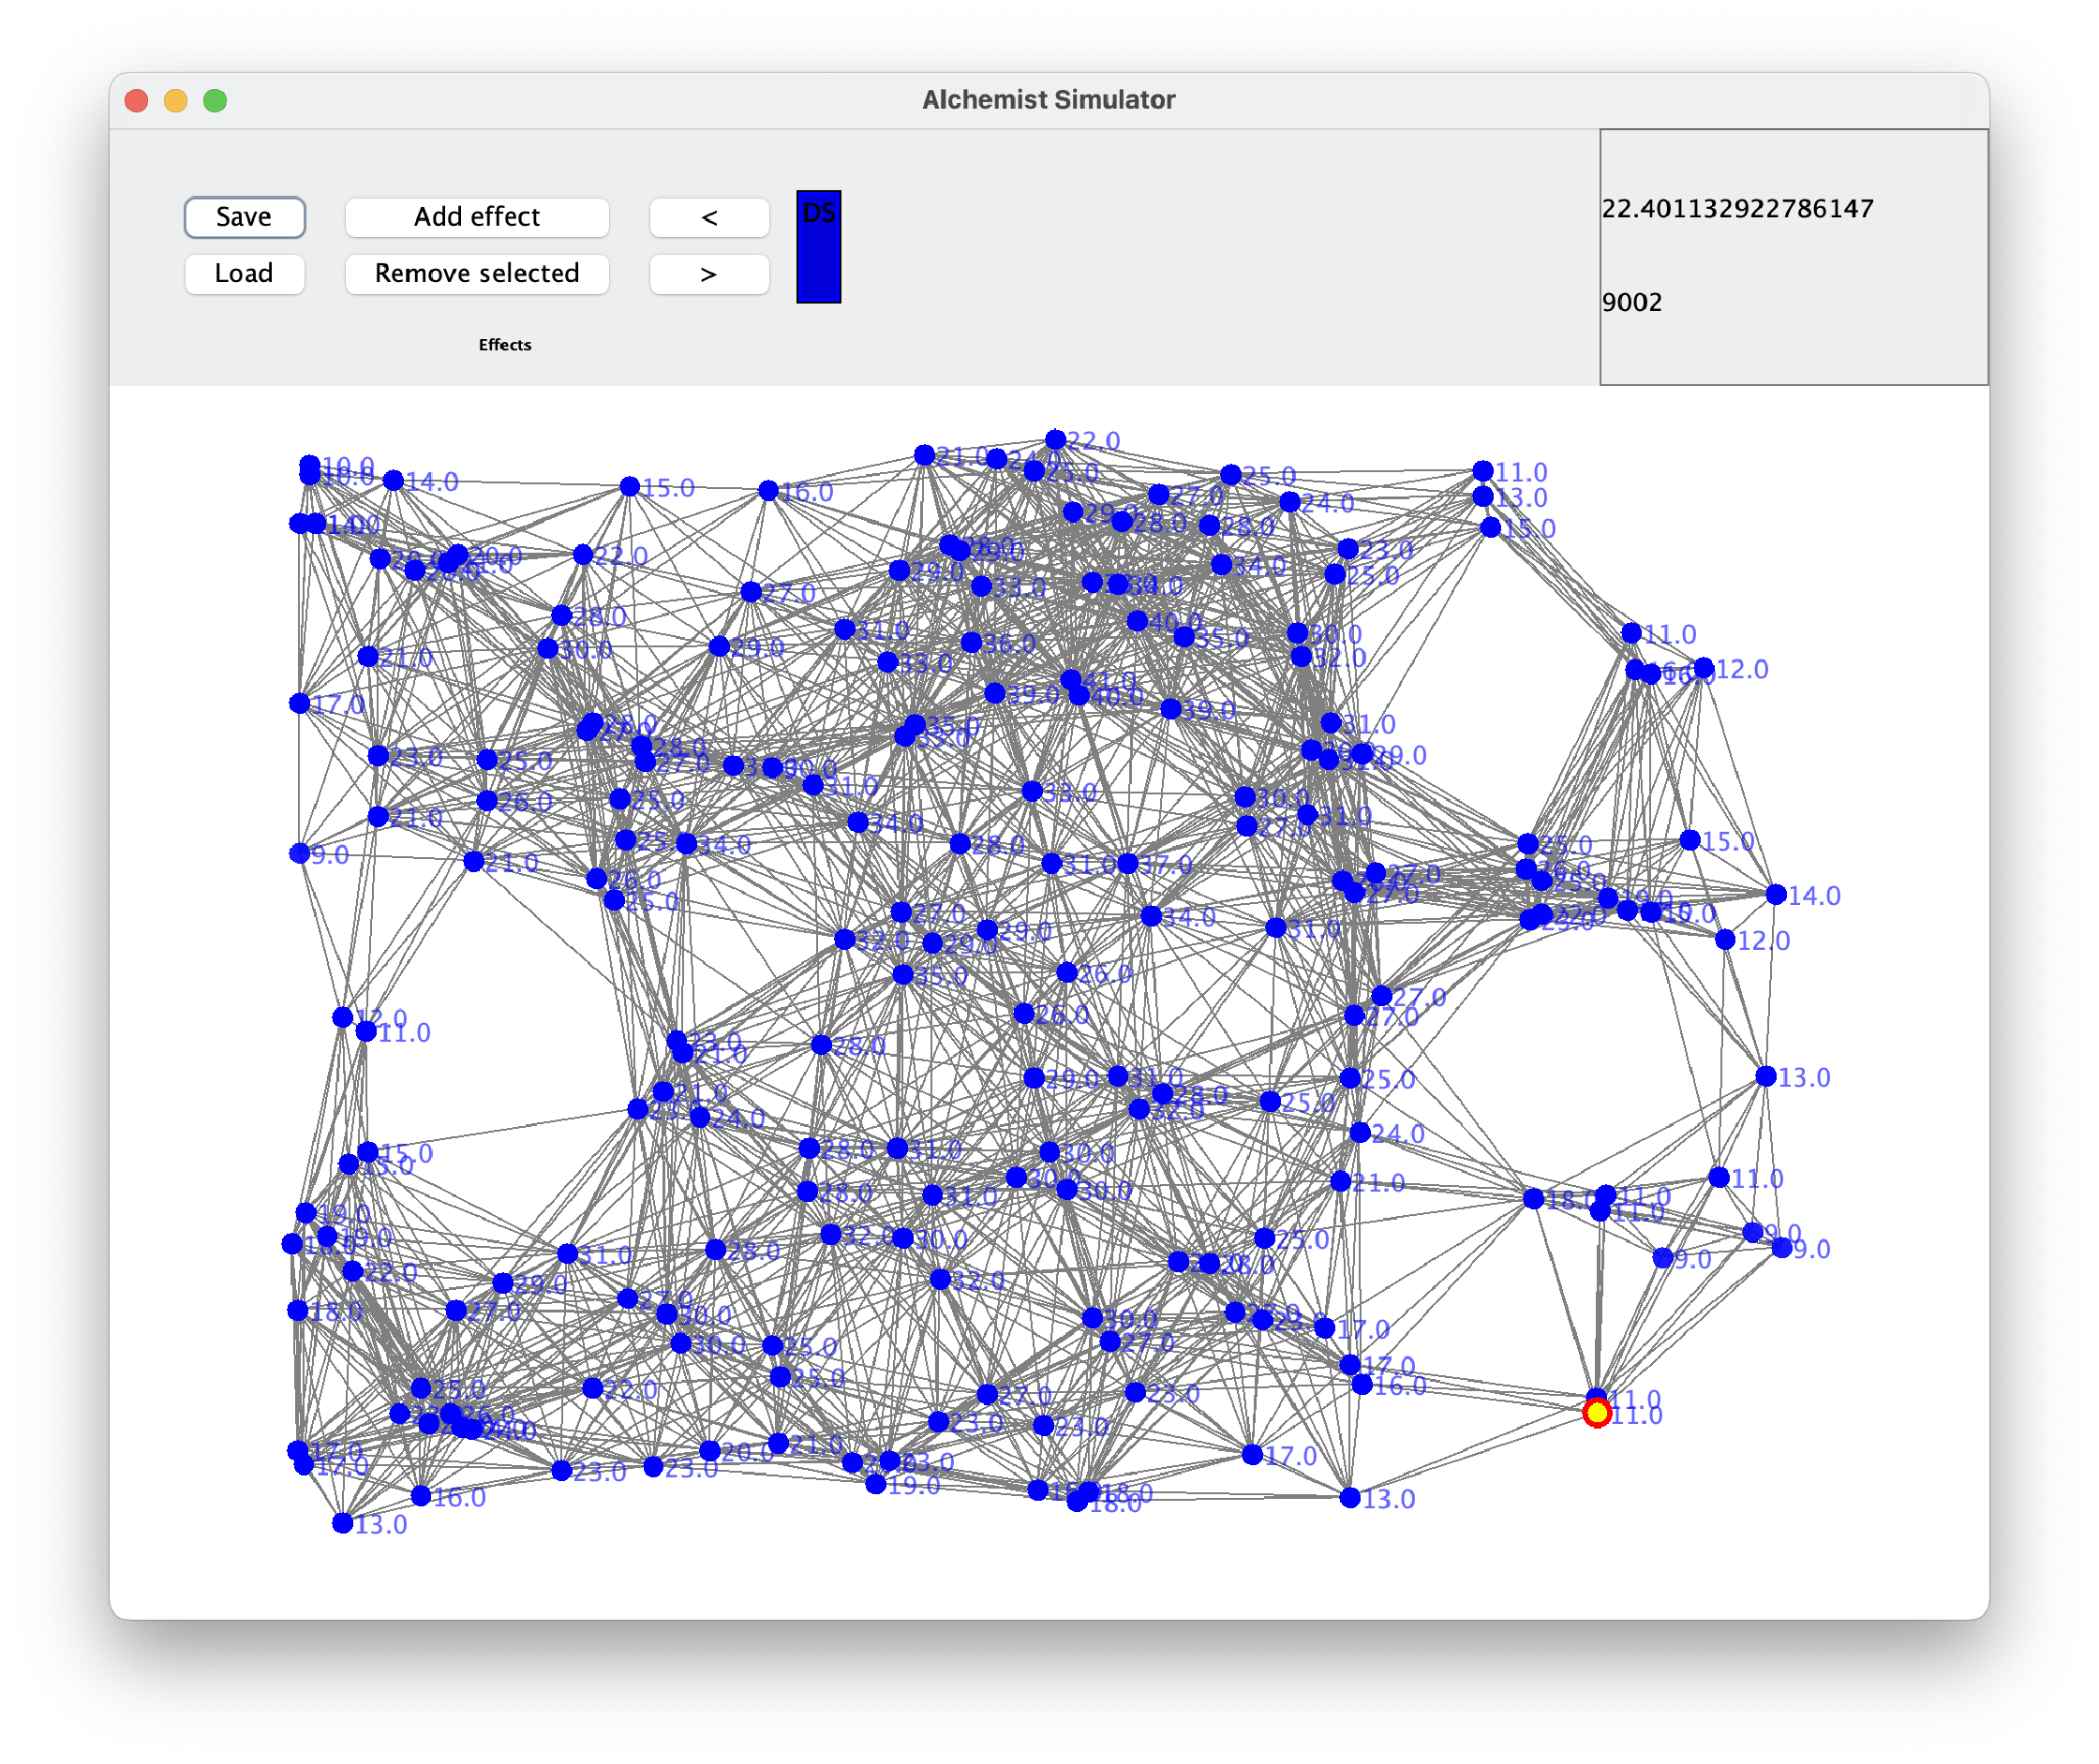
\includegraphics[width=0.8\textwidth]{figures/neighborCounterMoved}
    \caption{Neighbour Counter Simulation after moving some nodes.}
    \label{fig:neighbor-counter-moved}
\end{figure}

\paragraph{Gradient}
The second example is a simple gradient program in which the devices calculate the distance from a source node and
communicate it to the other nodes (\Cref{lst:gradient-example}).
The result is a map of the space in which each node has a value that represents the distance from the source node,
changing the colour of the nodes based on the distance from the source (seen as a square in \Cref{fig:gradient}).

\begin{lstlisting}[language=kt, caption={Gradient code example}, label={lst:gradient-example}]
context(LocalSensing,DistanceSensor)
fun Aggregate<Int>.gradientEntrypoint(): Double = gradient(sense("source"))

context(DistanceSensor)
fun Aggregate<Int>.gradient(source: Boolean): Double =
    share(POSITIVE_INFINITY) {
        val dist = distances()
        when {
            source -> 0.0
            else -> (it + dist).min(POSITIVE_INFINITY)
        }
    }
\end{lstlisting}

\begin{figure}[ht!]
    \centering
    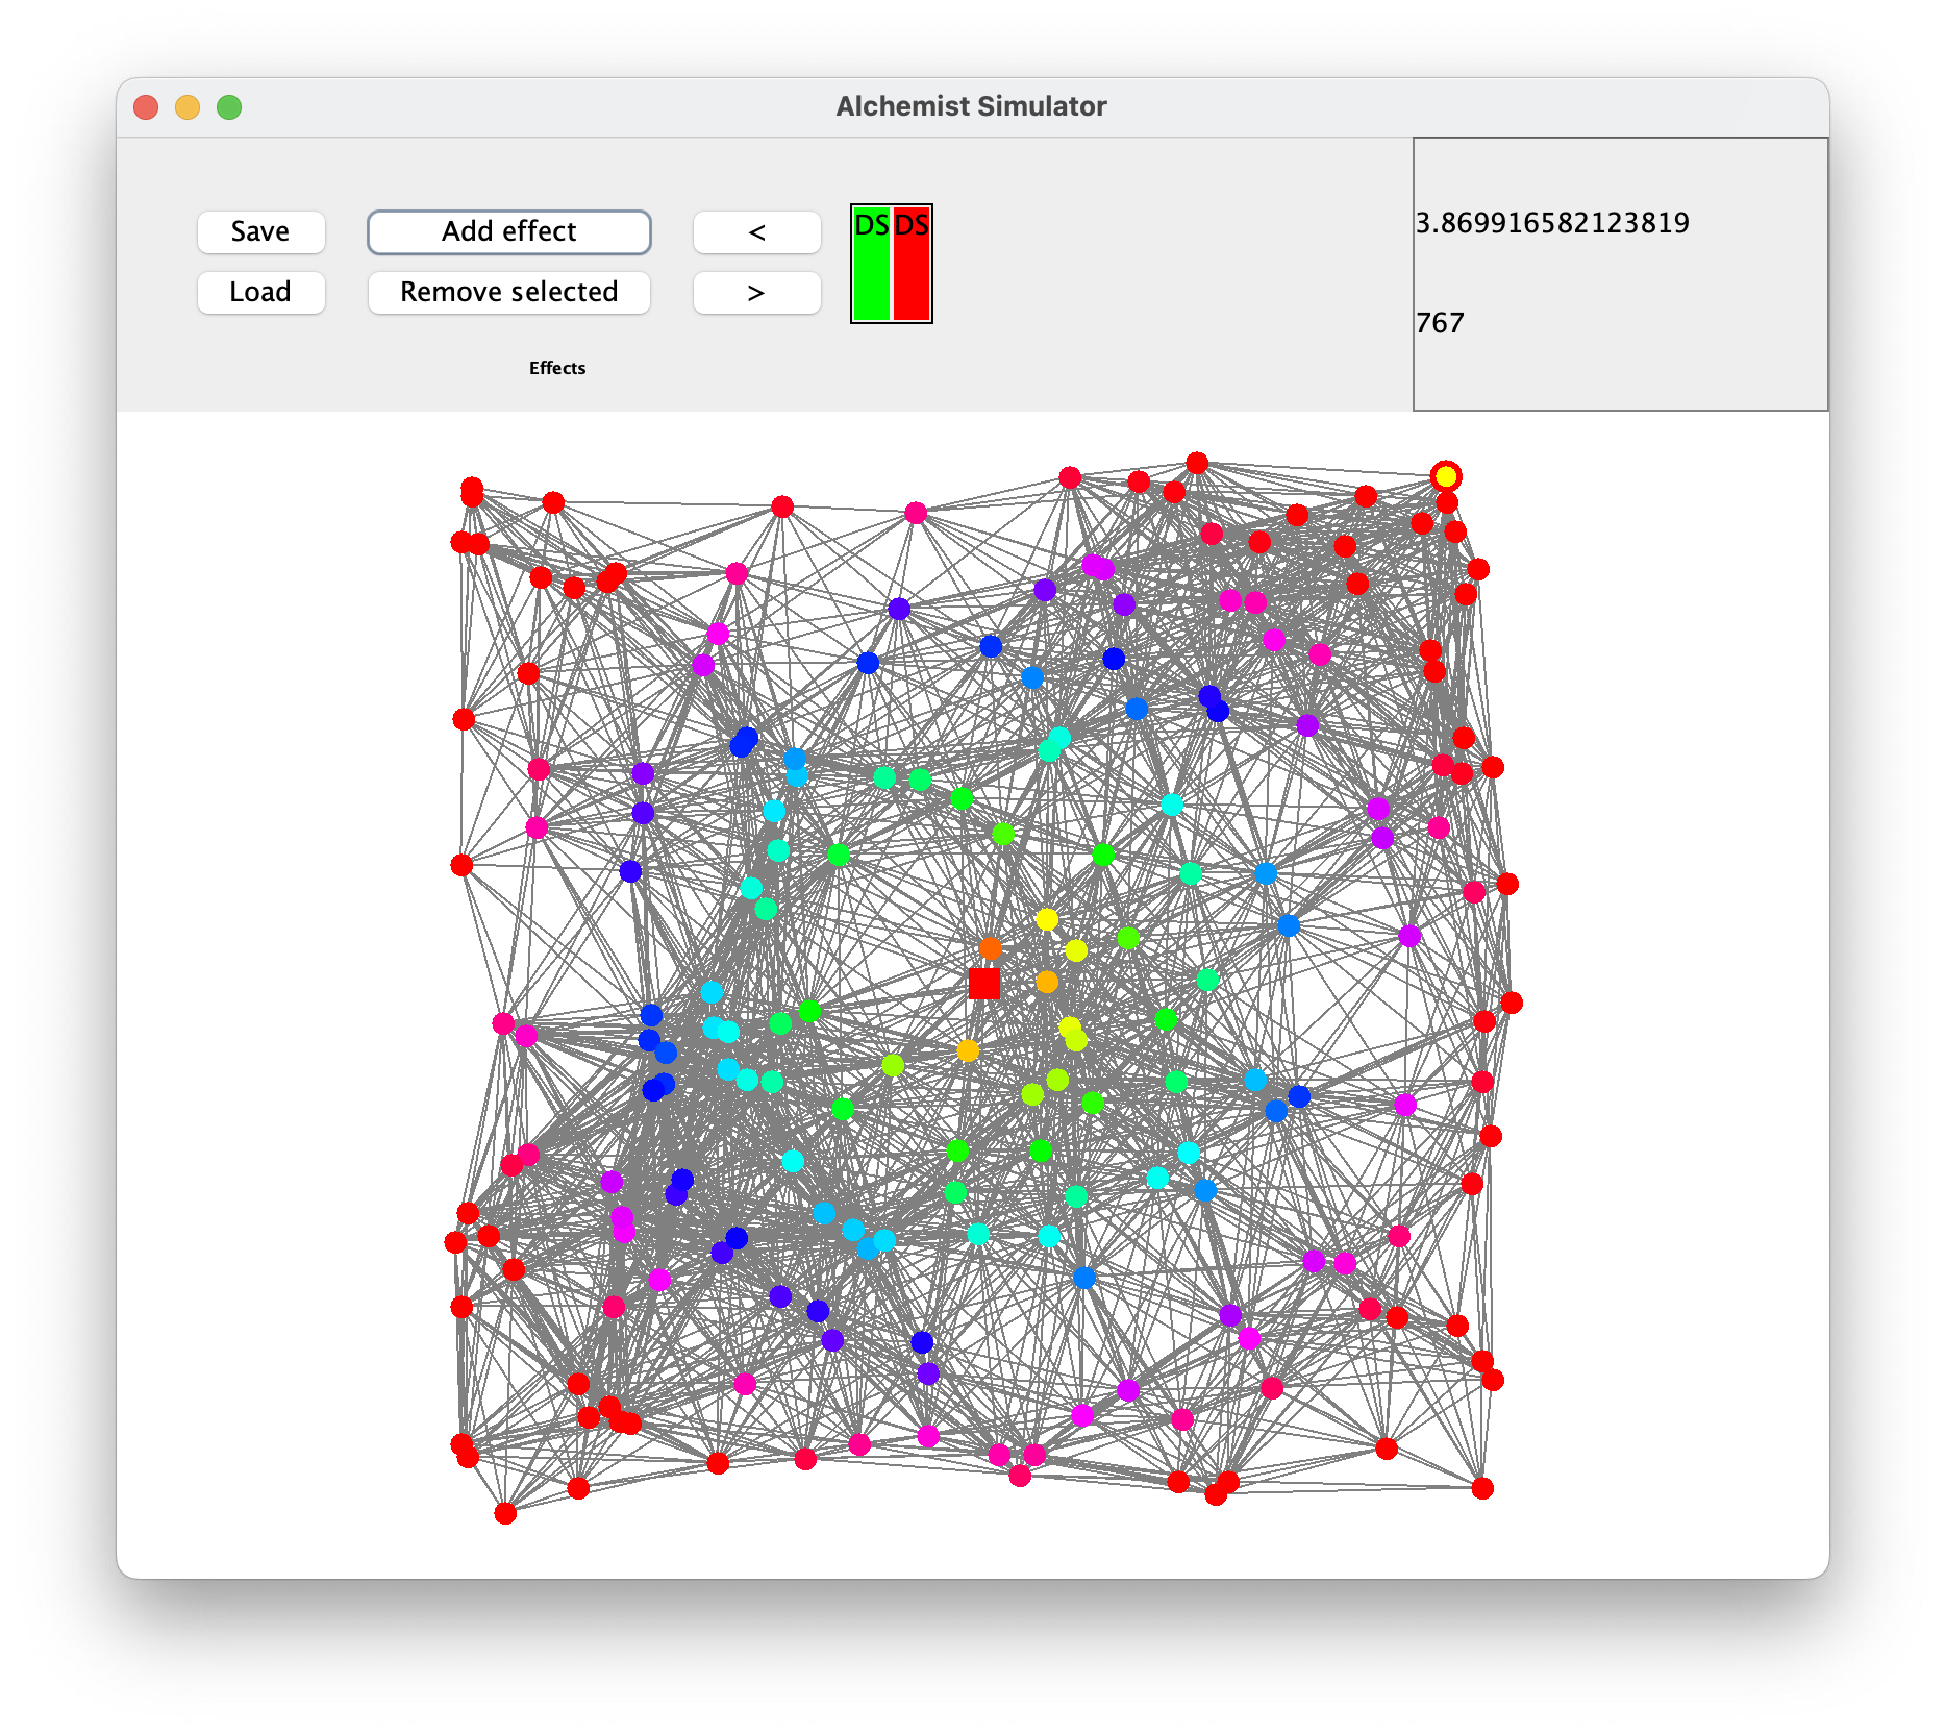
\includegraphics[width=0.8\textwidth]{figures/gradient}
    \caption{Gradient Simulation.}
    \label{fig:gradient}
\end{figure}

Also in this case, the simulator gives the opportunity to move the nodes around the environment, and the distance from
the source is updated in real-time (\Cref{fig:gradient-moved}).

\begin{figure}[ht!]
    \centering
    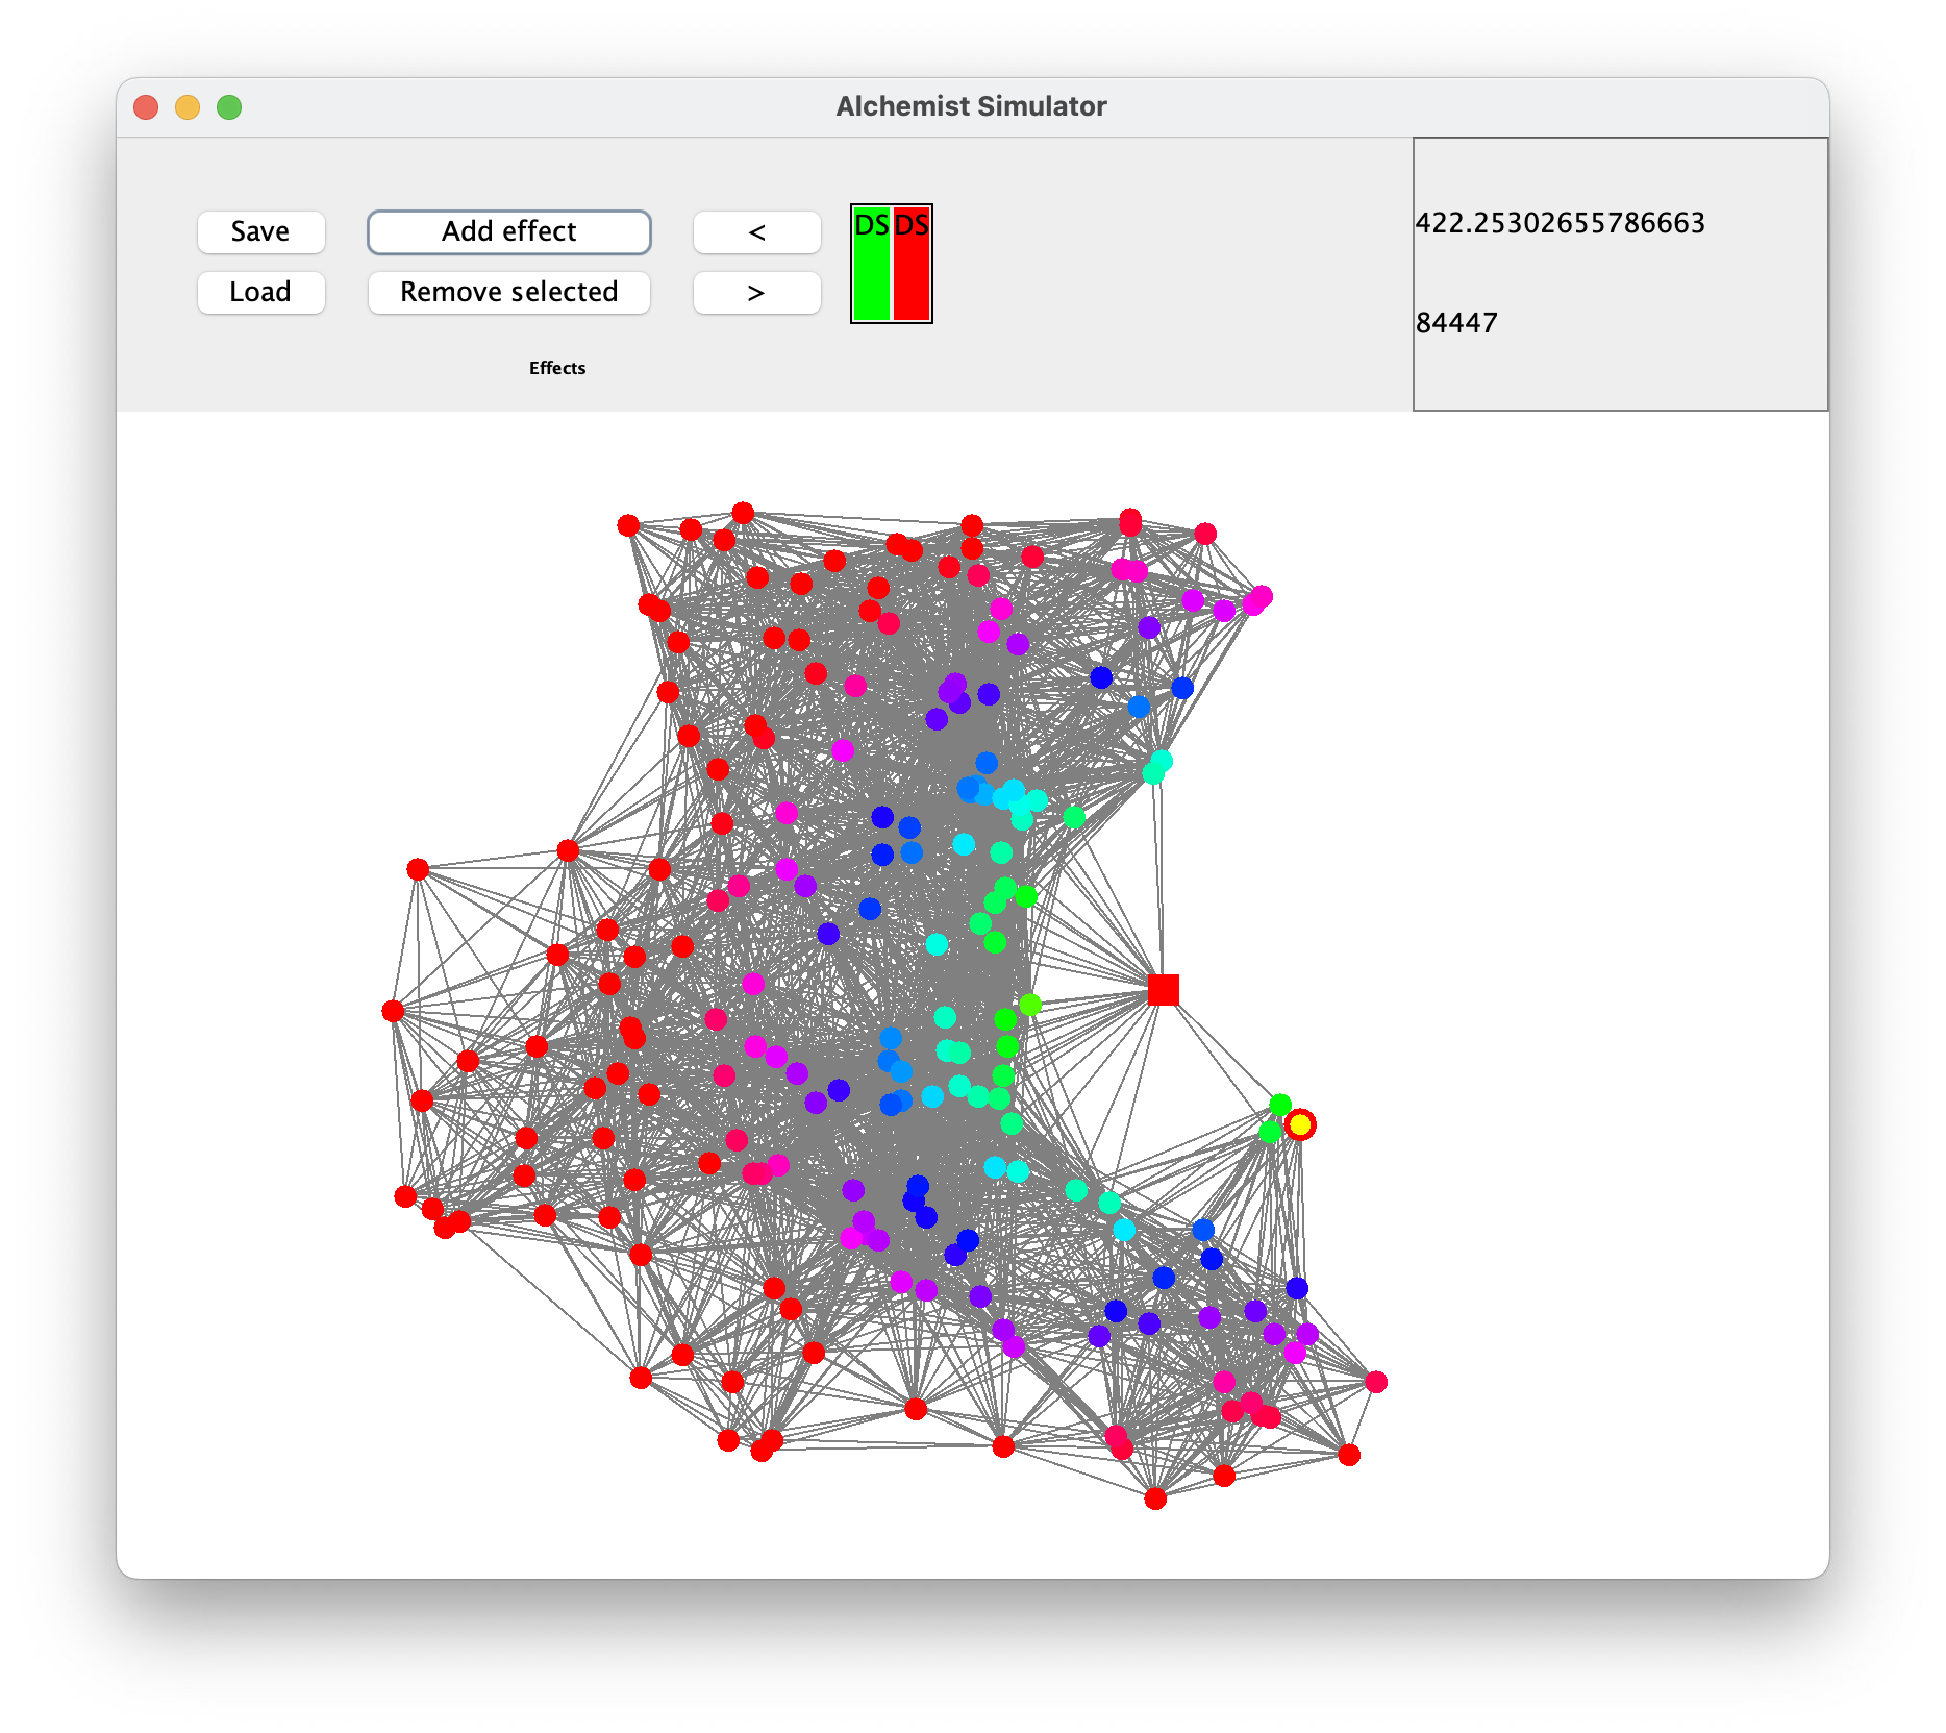
\includegraphics[width=0.8\textwidth]{figures/gradient-moved}
    \caption{Gradient Simulation after moving the root and some nodes.}
    \label{fig:gradient-moved}
\end{figure}

\paragraph{Channel with Obstacles}
The third example is a program a bit more complex, recreating a communication pathway (channel) within a distributed
system where data transmission is impeded or affected by various obstacles.
These obstacles could include network congestion, latency, limited bandwidth, or even physical barriers in certain
distributed computing environments.
In the context of aggregate computing, where computations are performed collectively by a network of interconnected
devices or nodes, such obstacles can significantly impact the efficiency and effectiveness of communication and data exchange among the nodes.

From a source node to a target node, the goal is to find a minimum path that avoids obstacles and is the most efficient
in terms of communication letting the information flow through the network (\Cref{lst:channel-with-obstacles-example}).

\begin{lstlisting}[language=kt, caption={Channel with Obstacles code example}, label={lst:channel-with-obstacles-example}]
context(LocalSensing, DistanceSensor)
fun Aggregate<Int>.channelWithObstacles(): Boolean =
    if (sense("obstacle")) {
        false
    } else {
        channel(sense("source"), sense("target"), channelWidth = 0.5)
    }

context(DistanceSensor)
fun Aggregate<Int>.channel(source: Boolean, target: Boolean, channelWidth: Double): Boolean {
    val sourceDist = gradient(source)
    val targetDist = gradient(target)
    val distBetween = distanceBetween(source, target)
    return !((sourceDist + targetDist).isInfinite() && distBetween.isInfinite()) &&
            sourceDist + targetDist <= distBetween + channelWidth
}
\end{lstlisting}

As shown in \Cref{fig:channel}, the channel (in green) is gradually created from the source (in yellow) towards the
target (in blue), and the obstacles (red) influence the trajectory of the channel, as expected.

\begin{figure}[ht!]
    \centering
    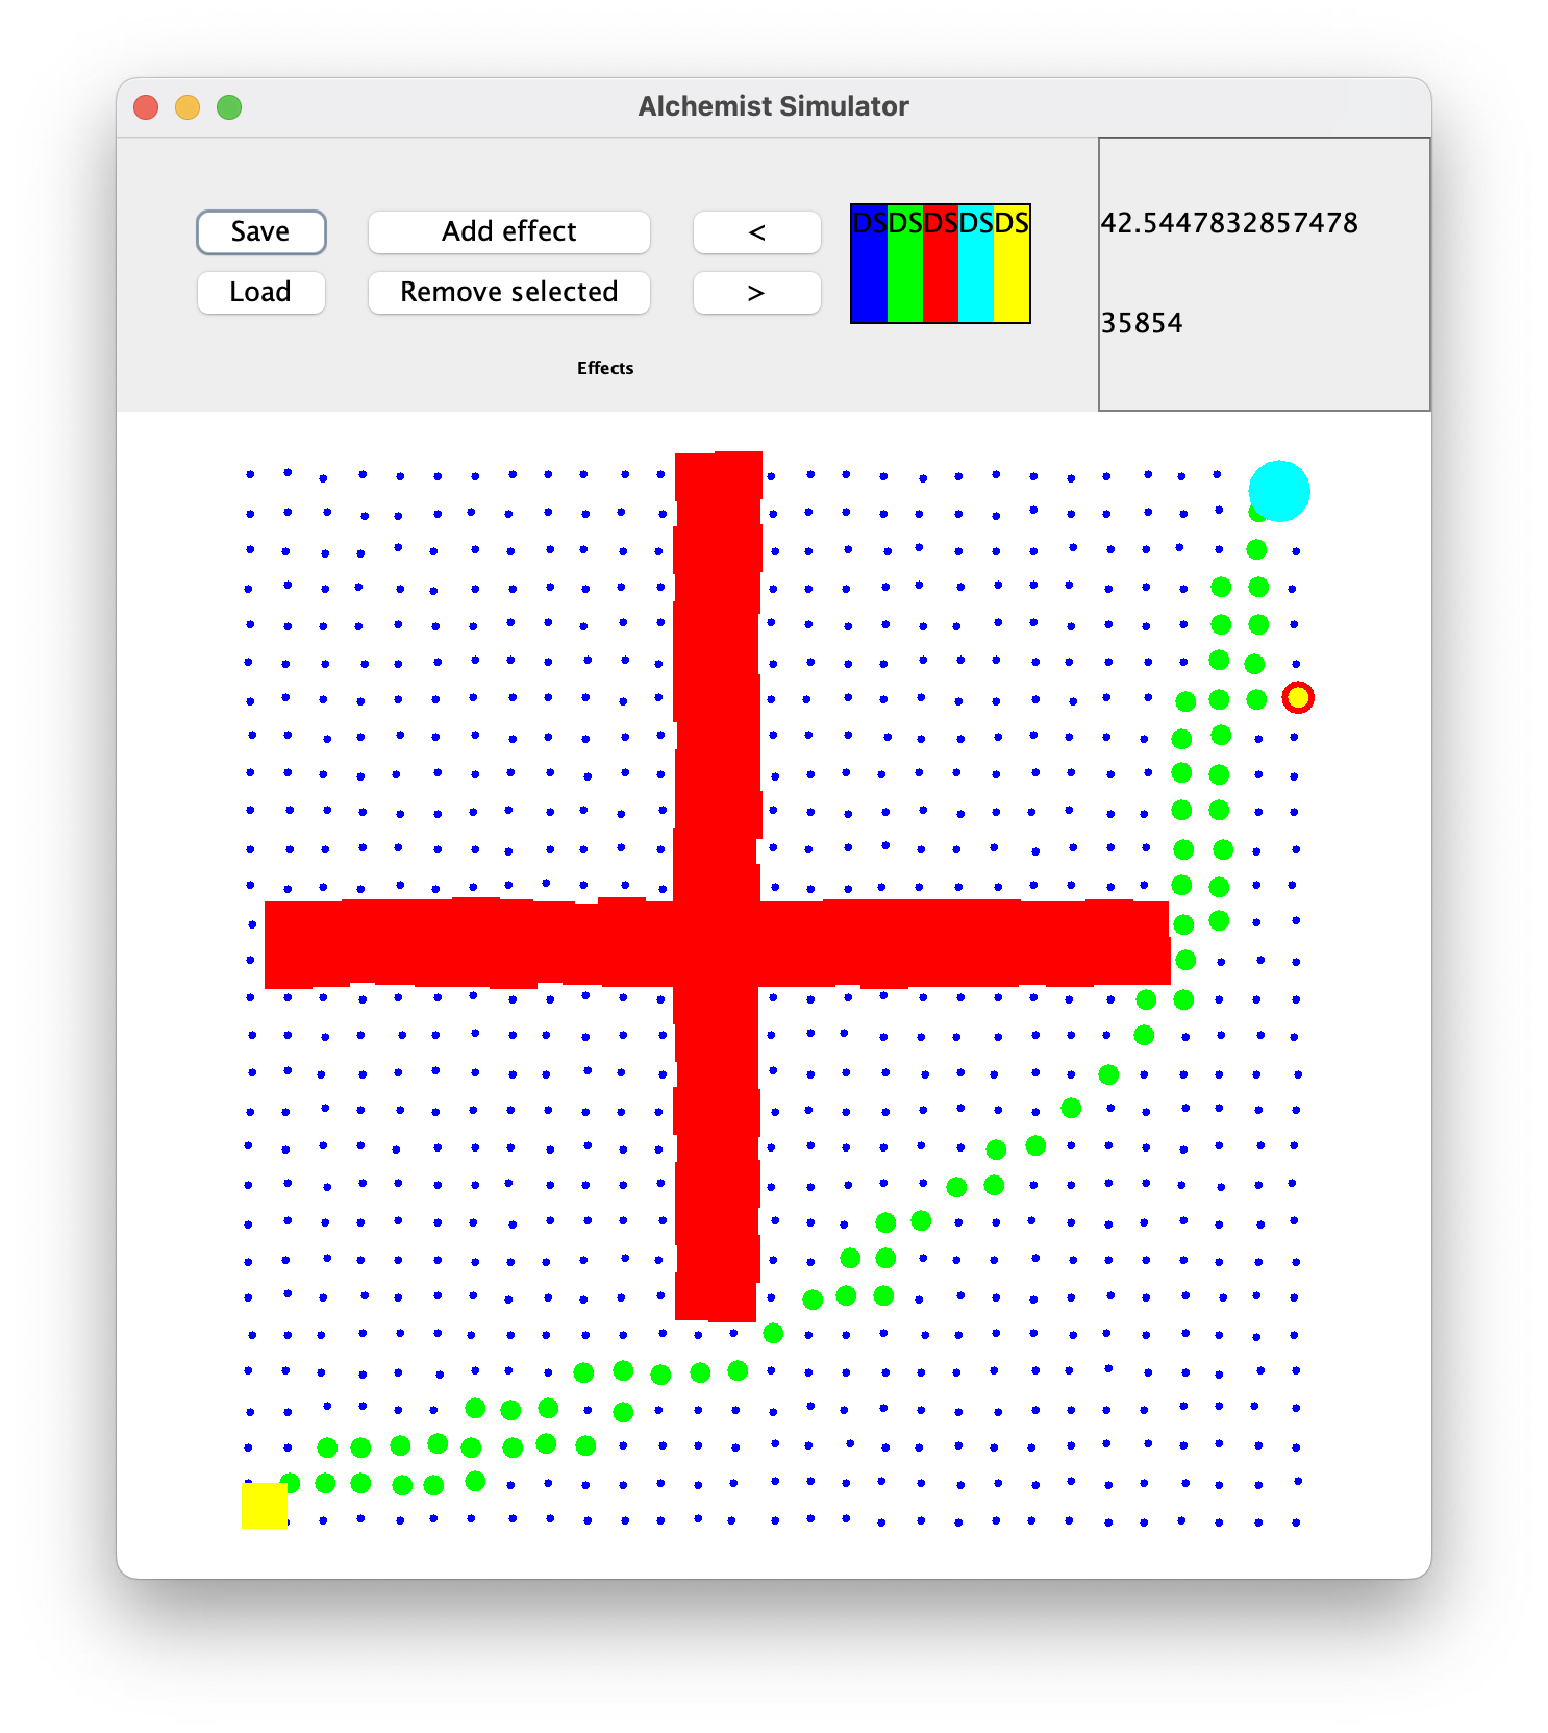
\includegraphics[width=0.6\textwidth]{figures/channel}
    \caption{The resultant simulation of the channel with obstacles.}
    \label{fig:channel}
\end{figure}

\section{Performance / Comparison}
\label{sec:performance-/-comparison}
To have a clear understanding of the performances of the new implementation, it is necessary to compare it with the
\emph{ScaFi} and \emph{Protelis}' incarnations.
The comparison is made by running the same simulations on each incarnation and comparing the results.
The simulations are run on the same machine to ensure that the comparison is fair and that the differences are due to the
implementation and not to the hardware.

The performance of the new language has been evaluated through the implementation of 5 types of tests:
\begin{enumerate}
    \item Simple \textbf{state change} of the device, to represent the variation over time of the field;
    \item A \textbf{counter of the neighbours}, to represent the variation of the space;
    \item A \textbf{gradient}, which is a particular case of space-time variation, in which the value of a node is a
        function of the distance from a node considered as a source;
    \item A \textbf{channel with obstacles}, to represent the presence of obstacles in space that influence the communication between nodes;
    \item Simple \textbf{branching} operations, as it has been noticed that branching could be one of the most expensive operations in terms of execution time.
\end{enumerate}

Each test has been run with the same parameters in the three different incarnations with three different simulated times
inside the \emph{Alchemist} simulator, and the results have been analysed and will be further discussed in this section.

\paragraph{Machine Specifications}
The results that will be presented have been obtained by running the simulations on a machine with the following specifications:
\begin{itemize}
    \item \textbf{Processor}: Intel(R) Core(TM) i9-14900KF;
    \item \textbf{RAM}: 64GB 4800mhz;
    \item \textbf{OS}: Linux Manjaro;
\end{itemize}

Other runs have been made on a different machine to ensure that the results are consistent across different hardware,
the machine used is the same as the tests one.

\paragraph{Foreword}
During the evolution of this thesis, it has been noticed that the current implementation of the alignment in \emph{Collektive}
may not be the optimal, as explained in \ref{sec:alignment}, and therefore the results could be influenced by this.
A way to implement a faster check on the alignment has been found, and it will be implemented in the future to have a more accurate comparison.

\paragraph{Field Evolution}
The first test has been implemented using the \texttt{repeat} construct.
It doesn't need any particular setup, as it is a simple state change of the device.

From the results, it is possible to see that the \emph{Protelis} implementation is faster than the \emph{Collektive} one,
which in turn is faster than the \emph{ScaFi} implementation.
%todo

\paragraph{Neighbour Counter}

\paragraph{Gradient}

\paragraph{Channel with Obstacles}

\paragraph{Branching}

\section{Discussion}

